75. $y=\sqrt{(1-2x)^2}-3=|2x-1|-3=\begin{cases}2x-4,\ x\geqslant\cfrac{1}{2}\\ -2x-2,\ x<\cfrac{1}{2}.\end{cases}$
$$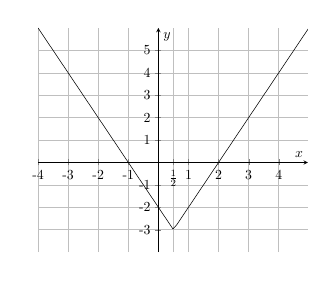
\begin{tikzpicture}[scale=0.5]
\begin{axis}[
    axis lines = middle,
    grid=major,
    legend pos={south west},
    xlabel = {$x$},
    ylabel = {$y$},
    ymin=-4,
    ymax=6,
    xtick={-3, 0.5, -4, -1, 1, 4,3, 6,-2,2,8},
    xticklabels={-3,  $\frac{1}{2}$, -4, -1, 1, 4,3, 6,-2,2,8},
    ytick={-3, -2, 1, -1,3,5,2,4},
    yticklabels={-3, -2, 1, -1,3,5,2,4}            ]
	\addplot[domain=-4:8, samples=100, color=black] {abs(2*x-1)-3};
%\addplot[domain=-3.1:2.5, samples=100, color=red] {70*abs(1-2*abs(abs(x)-2))-10*x^2+10*x-70};
	%\addlegendentry{$\text{Рис. 1}$};
\end{axis}
\end{tikzpicture}$$
Полученный треугольник является равнобедренным, высота, опущенная из его вершины, равна 3, как и основание. Пусть искомый радиус равен $R,$ тогда расстояние от центра окружности до основания равно $3-R$ и по теореме Пифагора $(3-R)^2+\left(\cfrac{3}{2}
ight)^2=R^2,\ 9-6R+R^2+\cfrac{9}{4}=R^2,\ R=\cfrac{15}{8}.$\\
